\documentclass[a4paper]{article}

% Essentials
\usepackage[utf8]{inputenc}
\usepackage[english]{babel}
\usepackage{hyperref}
\usepackage[table]{xcolor}
%\usepackage{latexsym,graphicx,graphics,epsfig}


% Hyperlinks
\hypersetup{
    colorlinks,
    linkcolor={red},
    citecolor={blue},
    urlcolor={blue}
}

% Optional but very useful
\usepackage[tmargin=3.5cm, bmargin=3.5cm, lmargin=3cm, rmargin=3cm]{geometry}
\usepackage{amsmath,amsthm,amsfonts,amssymb}
\usepackage{graphicx}
\usepackage{multicol}
\usepackage{float}
\usepackage{enumitem}
\usepackage{tabularx,booktabs,multirow}
\usepackage{longtable}
\usepackage{url}
\usepackage{enumitem}
\usepackage{todonotes}
\usepackage{caption}

% Title
\title{Excel Constraints}
\date{\today}

% Indentation
\setlength\parindent{0pt}

\begin{document}

\maketitle

% Content

\section{Use cases} % (fold)
\label{sec:use_cases}
There are different ways that learned constraints could be used in practice:

\begin{itemize}
	\item Find mistakes
	\item Suggest a formula for a specific field
	\item Suggest a next value
	\item Find structure and functions in a plain text sheet (such as a csv)
\end{itemize}

% section use_cases (end)

\section{Desired output} % (fold)
\label{sec:demo_example}
The annotated example (fig.~\ref{fig:demo}) demonstrates the most used constraints in Excel which we aim to identify automatically.

% section demo_example (end)
\begin{description}
	\item[Aggregates] Aggregate functions like sum, max, average, ... that reduce a range to a value
	\item[Conditional aggregates] Aggregates that use a filter on their input
	\item[Series] Ranges of integer numbers, ascending or descending (a special case of a permutation)
	\item[Lookups] Exact or fuzzy lookups that use a key to find a corresponding value
	\item[Ranks] Uses a range and a value to determine an order over elements
	\item[Structural constraints] Foreign keys to test value consistency between ranges
	\item[Previous] Uses row values and the previous value to compute the current value
\end{description}

Generally these constraints can be subdivided into:

\begin{itemize}
	\item Row constraints
	\item Column constraints
	\item Inter-table constraints
	\item Nested constraints
\end{itemize}

% section types_of_constraints (end)

\section{Approach} % (fold)
\label{sec:approach}

Currently we are considering a ModelSeeker like approach were ranges and values are generated and constraints tested upon them.
One option would be to use constraint-specific generators to avoid the explosion of the search space.
Meta-information would be used to find the most specific constraints.
A heuristic could use various information to determine which learned constraints are useful.

% section approach (end)

\begin{figure}
  \centering
    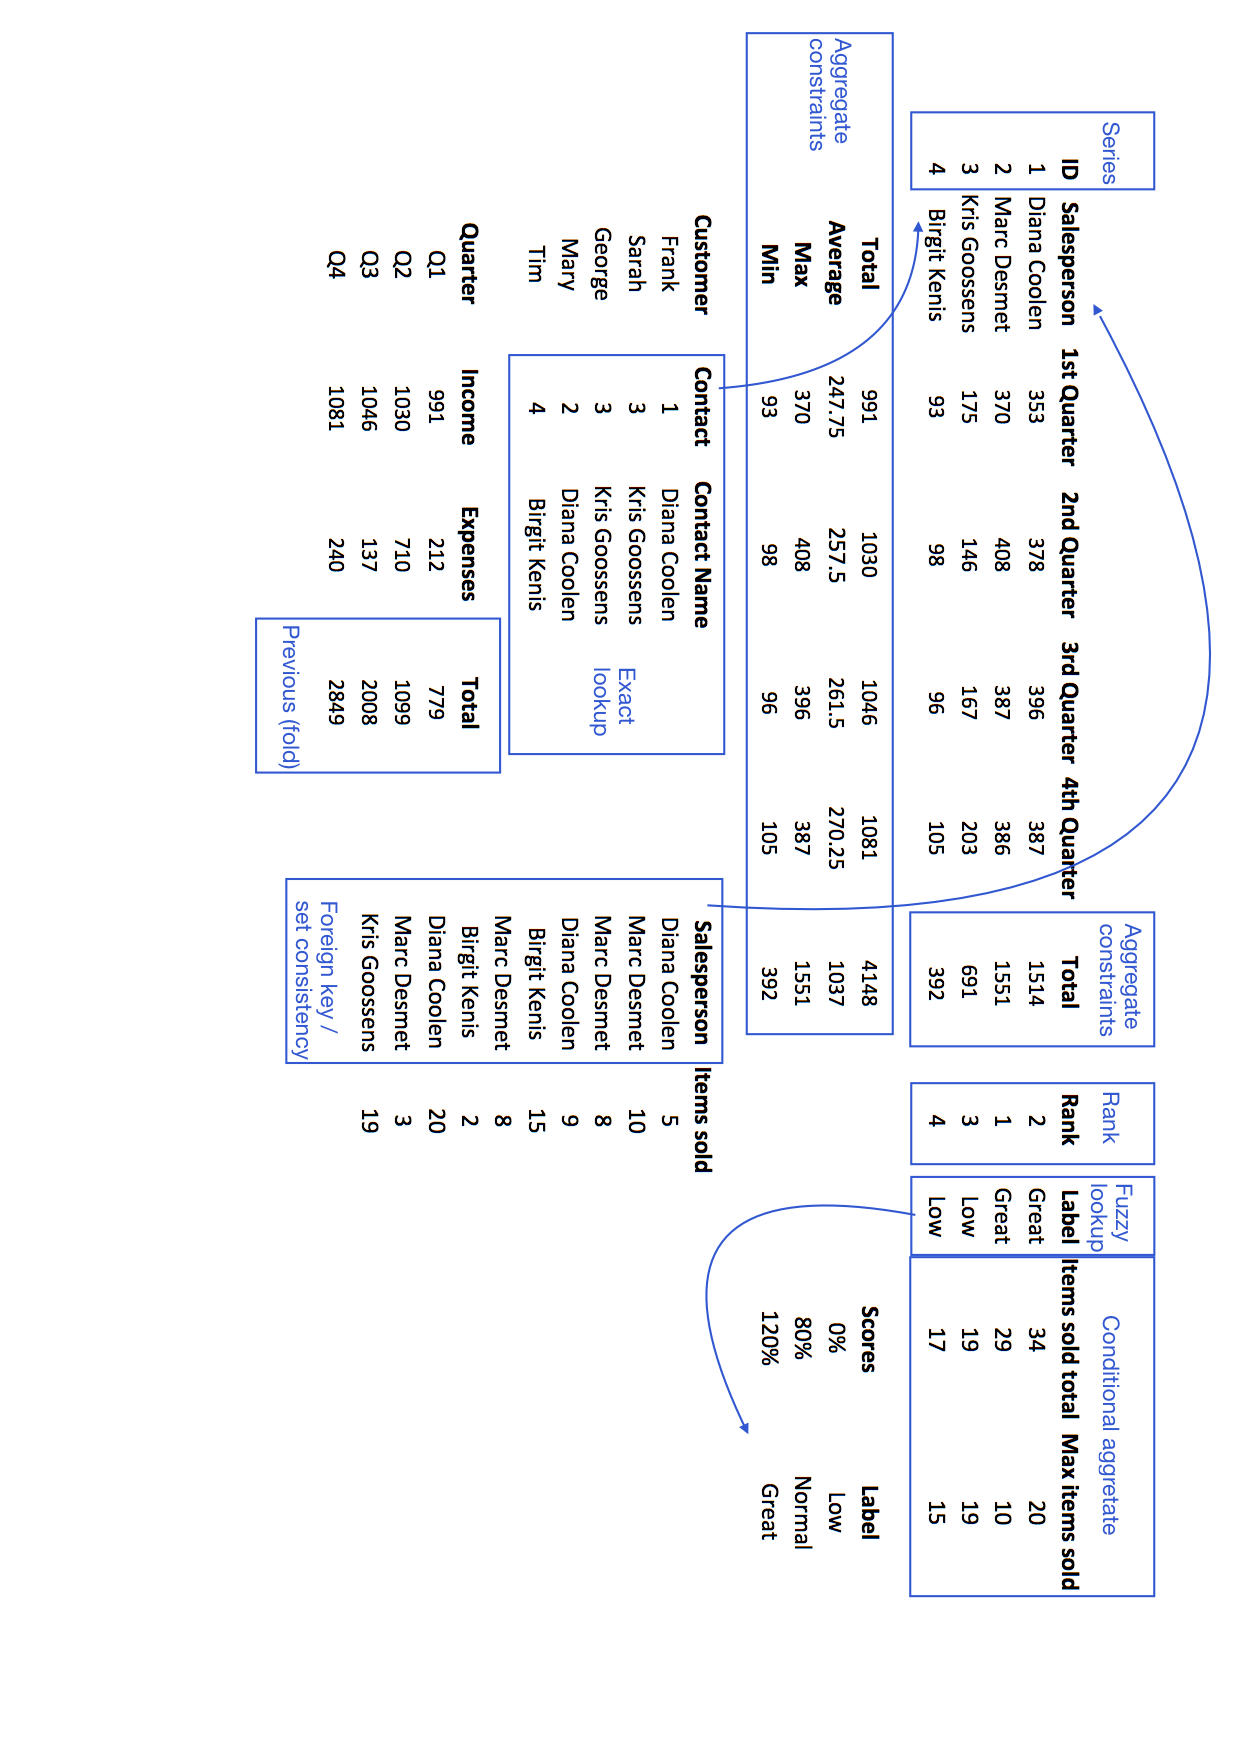
\includegraphics[width=1\linewidth]{../Demo.png}
  \caption{Demo example}
  \label{fig:demo}
\end{figure}

\end{document}